\section{Two-layers ReLU}

Data $x_j \in \R^d$ and labels $y_j \in \R$, $j=1,..,n$

First layer $w_i \in \R^d$, second layer $\alpha_i \in \R$, $i=1,..,m$

$\step>0$ step-size, $\reg$ regularization

\begin{equation}
	 \mathcal{L}(W, \alpha) = \sum_{j=1}^n \bigg( \underbrace{\sum_{i=1}^m \max(0, w_i^\top x_j) \alpha_i}_{\text{Network's Output}} - y_j \bigg)^2 + \underbrace{\lambda \sum_{i=1}^m \| w_i \|^2_2 + \alpha_i^2}_{\text{Weight Decay}}
\end{equation}


\textbf{Discret time.}

Full-batch gradient descent

\begin{equation}
	(W, \alpha)_{t+1} = (W, \alpha)_t - \step \nabla \mathcal{L}((W, \alpha)_t)
\end{equation}

Implicit

\begin{equation}
	\param_{t+1} = \argmin_{\param} \mathcal{L}(\param) +\frac{1}{2\step} \norm{\param - \param_t}
\end{equation}

\textbf{Continuous time.}

Taking $\step \to 0$, we get the gradient flow: $\frac{\dd \param_t}{\dd t} = - \nabla \mathcal{L}(\param_t)$. We make ReLU differentiable with $\sigma'(0)=0$ as justified in \citep{boursierGradientFlowDynamics2022}.

\subsection{Explicit gradient}

Take a two layer ReLU network with $m$ neurons. Each neuron has a trainable parameter $w_i \in \R^d$ and and a fixed output sign $\alpha_i \in \{-1, 1\}$. Each of the $n$ data points of dimension $d-1$ are augmented with a $1$, so each sample is of dimension $n$. Each sample $x_j$ is stored as a row $X \in \R^{n \times d}$  and is associated with a scalar label $y_j \in \R$.

The output of one neuron is: $x \in \R^d \rightarrow \max(0, \inp{w_i}{x}) \alpha_i$, shorthand $\inp{w_i}{x}_+ ~ \alpha_i$.

The output of a network of $m$ neurons on one data point is $f(x) = \sum_{i=1}^{m} \max(0, \inp{w_i}{x}) ~ \alpha_i$

We store the neuron trainable parameter $w_i$ as the columns of $W \in \R^{d \times m}$. The loss for $n$ data points

\begin{equation}
	F(W) = \frac{1}{n} \sum_{j=1}^{n} \left(f(x_j) - y_j\right)^2
\end{equation}

Discretized, unregularized gradient descent with $\lambda \in \R^+$ stepsize: (resolving the non differentiable points $\max(0, 0)$ with 0 as gradient)

\begin{equation}
	W^{t+1} = W^t - \lambda \nabla F(W^t)
\end{equation}

Taking $\lambda \rightarrow 0$, we get the gradient flow.

Explicit discret gradient:

\begin{equation}
	\frac{\partial F}{\partial \vw^t_i} = \frac{\alpha^t_i}{n} \sum_{j=1}^{n} e^t_j ~ s^t_{i, j} ~ \vx_j
\end{equation}

With real $e^t_j = f(W^t) - y_j$ the "signed error on input $j$"

With boolean $s^t_{i, j} = \mathds{1}_{\inp{\vw^t_i}{\vx_j} > 0}$ the "is neuron $i$ activating on datapoint $j$. The vector $\vs^t_{i} \in \{0, 1\}^n$ would be the activation pattern of neuron $i$ at time $t$.

Remark: the gradient of a neuron is a linear combination of the data points it activates.


\section{Convergence of mean-field networks}

\textbf{Mean-field limit}\citep{chizatGlobalConvergenceGradient2018}: For a sufficiently large width, the training dynamics of a NN can be coupled with the evolution of a probability distribution described by a PDE.

If [...] converges, with $m \rightarrow \infty$ (many-particle limit), our particles of interest converges to a Wasserstein gradient flow of F:

\begin{equation}
	\partial \mu_t = - \diver(v_t \mu_t) \text{ where } v_t \in - \partial F'(\mu_t)
\end{equation}

\begin{equation}
	\int_\paramS m(\param; x) \dd \mu(\param) = \frac{1}{m} \sum_{i=1}^{m} \inp{\vw_i}{\vx_j}_+ \alpha_i
\end{equation}

Remark: le 1/m c'est principalement pour être ok à l'infini. Dans le papier JKO \citep{carlierConvergenceEntropicSchemes2017} ils utilisent un vecteur de proba

Different ways to use a measure to represent the neurons of a two layer network:

\begin{itemize}
	\item $\paramS = \R^d \times \R$, measure $\mu = \frac{1}{m} \sum_{i=1}^{m} \dirac_{\param_i = (\vw_i, \alpha_i)}$, output of one neuron $m(\param=(\vw,\alpha); \vx) = \inp{\vx}{\vw}_+ \alpha$: (works, output matches discrete)
	\item $\paramS = \R^d$, measure $\mu = \frac{1}{m} \sum_{i=1}^{m} \alpha_i \dirac_{\param_i = \vw_i}$ output of one neuron $m(\param=\vw; \vx) = \inp{\vx}{\vw}_+$ (works)
	\item $\paramS = \R^d \times \R^d$, output of one neuron $m(\tilde{\vw}_+, \tilde{\vw}_-, \vx) = \inp{\tilde{\vw}_+}{\vx} - \inp{\tilde{\vw}_-}{\vx}$ (works, separate neg and positive)
	\item $\paramS = (S^{d-1} \times \R)$, output of one neuron $m((\vd, \tilde{\alpha}); \vx) = \tilde{\alpha} \inp{\vd}{\vx} = \tilde{\alpha}\  \mathds{1}_{\inp{\vd}{\vx}>0} $ (works), mapping: $\vd = \frac{\vw}{\norm{\vw}}$ and $\tilde{\alpha}=\norm{\vw} \alpha$. Gradient are not equal to discrete.
\end{itemize}

\subsection{Algorithm, discretize the measure's space}

Take a grid of $N$ points in $\paramS$, we can match the notation above by taking a neuron for each point of the grid $m=N$.

The grid currently dictate the neuron's scale, giving multiple choices.

\begin{equation}
	\mu(t+1) = \argmin_{\mu \in \mathcal{M}(\paramS)} F(\mu) + \frac{1}{2 \step} W_2(\mu; \mu(t))
\end{equation}



Take $\step \to 0$, get gradient flow. Take $m \to \infty$, get wasserstein gradient flow \citep{bachGradientDescentInfinitely2021}, and if it converges, it goes to the global optimal.

\section{Mean field rewritten results}
\subsection{direct result}

Minimization of a linear combination of ('neurons' $\{\phi(\theta)\}_{\theta \in \Theta}$) through an unknown measure $\mu$: $J^* = \min_{\mu \in \mathcal{M}(\Theta)} J(\mu) = R(\int \phi \dd \mu) + G(\mu)$

With $R$ a convex loss function and $G$ a convex regularizer, $\mathcal{M}(\Theta)$ the set of signed measures on the parameter space $\Theta$.

Discretize the measure into $m$ particles: $\min_{w \in \R^m \\\ \theta \in \Theta^m} J_m(w, \theta) = J( \frac{1}{m} \sum_{i=1}^{m} w_i \delta_{\theta_i})$

Proved: if WGF cvg, it cvg to global minimizer. If $(w^{(m)}(t), \theta^{(m)}(t))_{t>0}$ are gradient flows for $J_m$ then, with the corresponding measure $\mu_{m,t} = \frac{1}{m} \sum_{i=1}^{m} w^{(m)}_i(t) \sigma_{\theta_i^{(m)}(t)}$ (a WGF), $J(\mu_{m, t})$ cvg (with $m, t \rightarrow \inf$) to global minimizer of $J$.

p-Wasserstein distance between two measures $\mu, \nu \in \mathcal{P}(\R^d)$: $W_p(\mu, \nu)^p = \min_{\gamma \in \Pi(\mu, \nu)} \int |y - x|^p \dd \gamma(x, y)$

\subsection{simple result}

Cast the parameters $w \in \mathcal{W}^{d+1}$ into $r \in \R, \eta \in \mathcal{S}^d = {w \in \R^{d+1}, \norm{w}_2 = 1}$ with $w = r ~ \eta$. The two flows will have exactly the same dynamics.

Then measure $\nu= \frac{1}{m}\sum_{j=1}^{m} r^2_j \sigma_{\nu}$ satisfy this PDE : $\partial_t \nu_t(\eta) = -4 J(\eta | \nu_t) + \diver(\nu_t(\eta) \nabla J(\eta | \nu_t)) $ (so it's a WGF)

Prediction functions : $h = \frac{1}{m} \sum_{j=1}^{m} \psi(w_j) = \frac{1}{m}\sum_{j=1}^{m} r_j^2 \psi(\nu_j)$

Theorem 1: if by taking $m \leftarrow \inf$ at $t=0$, $\nu$ converges to $\nu_0$, then for any $t$, $\nu_{m, t}$ cvg to the unique WGF $\nu_t$.

Theorem 2: Take a $\nu_0$ with a support that includes all directions at initialization, if WGF $\nu_t$ cvg, it's to a global optimum.


\section{Simple example 2D setting, grid jko}

From one dimensional data, we add a dimension filled with ones to act as a bias for the first layer. The output of one ReLU neuron for one data point $(x, 1) \in \R^2$:

\begin{equation}
	w, b, \alpha \in \R \rightarrow \max(0, w x + b) \alpha
\end{equation}

The loss against labels $y_j \in \R$ using squared loss of the whole network of neurons is the double sum:

\begin{equation}
	 \mathcal{L} = \sum_{j=1}^n \left(\left(\sum_{i=1}^m \max(0, w_i x_j + b_i) \alpha_i \right)  - y_j \right)^2
\end{equation}

The mean-field limit of this network requires taking an infinite-width ReLU network where parameters are described by a measure $\mu$, and its output by an integral:

\begin{equation}
	\int_{\R^2} m((w, b); x) ~ \dd \mu((w, b))
\end{equation}
 
To simplify things, we restrict $\alpha_i$ to $\{-1, 1\}$ and to not be a trainable parameter anymore. We keep the same expressivity(as long as we provide both a positive($\alpha_i=1$) and negative($\alpha_i=-1$) version of the neuron) but this change will slightly alter the training dynamic in some cases. For example , we can match the output of one neuron (of the original network) by simply scaling the first layer by the seconder layer ($\alpha$):

\begin{equation}
	\max(0, w_i x + b_i) \alpha_i = \max\left(0, |\alpha_i|(w_i x + b_i)\right) \ \text{sign}(\alpha_i)
\end{equation}

Our network with restricted $\alpha_i$ would describe this neuron using only two trainable parameters: $(|alpha_i| w_i, |\alpha_i| b_i)$ and fix its sign in the output.

The measure is on the parameter space. In order to do simulations we discretize the parameter space, by taking a uniform grid in $\R^2$ centered on $(0, 0)$: $(w_i, b_i)_{i=1, \dots m}$

We can see that we have the same output and expressivity as the regular ReLU network by taking a measure $\mu = \sum_{i=1}^{m} p_i \dirac_{\param_i = \vw_i}$ with ($\sum_i p_i=1$) and $m((w_i, b_i); x) = \max(0, w_i x + b_i) \alpha_i$, we have this equality:

\begin{equation}
	\int_{\R^2} m((w, b); x) \dd \mu((w, b)) = \sum_{i=1}^{m} \max(0, w_i x_j + b_i) \alpha_i p_i
\end{equation}

In this case, the first layer is fixed: the change of direction($\frac{-b_i}{w_i}$) and slope $(w_i)$ of a neuron is described by a mass displacement from point A to point B. 

The movemement is described by a PDE and simulated on a grid. Each point $i$ of the grid has a weight $p_i \in \R$, and as a whole $p \in \R^m$ is the discretized distribution.

The same wasserstein gradient flow can be computed by this step:

\begin{equation}
	\mu(t+1) = \argmin_{\mu \in \mathcal{M}(\paramS)} F(\mu) + \frac{1}{2 \step} W_2(\mu; \mu(t))
\end{equation}

We tried different ways of computing the Wasserstein Gradient Flow. 

\begin{itemize}
	\item JKO stepping: entropic approximation on a fixed grid. Pros: not very dependant on dimension $d$. Cons: add another loop and more parameters to fine tune, introduce diffusion.
		\item Sliced Wasserstein: Pros: midly dependant on $d$ without diffusion. Differentiable with pytorch. Cons: Parameters to tune, distance to true WS distance has to be studied
		\item Direct EMD distance from POT library. Pros: differentiable with pytorch. Cons: Might be slow with $d$
\end{itemize}

Preliminary results using the EMD distance indicate no particular differences between the gradient flow and the wasserstein gradient flow.


\section{2 pts example}

On étudie un problème en une dimension, avec analogie possible entre l'évolution de deux neurones ReLU(à activation fixe) dans $\R^d$ et l'évolution de $x$(qui active une donnée et estime un label '$4$' et $y$ qui n'active aucune donnée.

$(x^{(0)}, y^{(0)}) = 0, 1$

\begin{equation}
	\min_{x,y \in \R} \underbrace{\frac{1}{2}(x - 4)^2}_{f(x, y)}
\end{equation}

En étudiant en détail une étape de prox, càd:

\begin{equation}
	(x^{(t+1)}, y^{(t+1)}) = \argmin_{(x, y)} f(x, y) + \frac{1}{2 \gamma} \dd((x,y),(x^{(t)}, y^{(t)}))
\end{equation}

Avec $\gamma > 0$ la taille du pas qui caractérise en gros à quel point la solution de l'argmin ($(x,y)^{(t+1)}$ peut s'éloigner de l'initialisation/itéré précédent ($(x,y)^{(t)}$

\textbf{petit résumé de la suite.}

On trouve que: avec d = frob/eucli (i.e. $(x-x^{(t)})^2 + (y-y^{(t)})^2$), avec plusieurs étapes on converge toujours(i.e. $\forall \gamma > 0$) vers $(x=4, y=1)$ : $y$ est constant.

Avec d = wasser($W^2_2$) (le plus petit entre frob et $(x-y^{(t)})^2 + (y-x^{(t)})^2$)

-\verb|->| en une étape: la limite pour un pas infini est $(x=4, y=0)$. On déplace donc le point $y$ qui a une dérivée nulle pour la fonction $f$ à minimiser.

-\verb|->| plusieurs étapes: quasiment idem, voir les schémas

\subsection{détail wasser}

Préreq(partie suivante): $w_2$ avec mesures somme de diracs uniforme \verb|->| pb de permutation.

On trouve facilement que l'assignement est l'identité si $x \leq  y$ et on inverse dans l'autre cas (avec deux solutions pour l'égalité). On peut réécrire l'argmin avec la distance de wasserstein:

\begin{equation} \label{eq:argwass}
	(x^{(t+1)}, y^{(t+1)}) = \argmin_{(x, y)} \frac{1}{2}(x-4)^2 + \frac{1}{2 \gamma} \left[ \one_{x \leq y} ~ \left((x-x^{(t)})^2 + (y - y^{(t)})^2\right) + \one_{x > y} ~ \left((x-y^{(t)})^2 + (y - x^{(t)})^2\right) \right]
\end{equation}

\emph{Dans \cref{eq:argwass}, soit on paie le coût de transporter $x^t$ vers $x$ et $y^t$ vers $y$ (si $x^t < y^t$, car c'est le plus efficace dans ce cas), soit on paie le transport de $x^0$ vers $y$ et $y^0$ vers $x$.}

\subsection{wasserstein: détails de la première étape}

\textbf{Pour $\gamma < 1/3$.}

la première étape de prox sera identique qu'importe la distance utilisé, car $x^{(1)} \leq y^{(0)}$(avec un petit pas, il n'est pas possible d'obtenir une solution plus loin que $y^{(0)}$. \cref{eq:argwass} devient:

\begin{equation}
	(x^{(t+1)}, y^{(t+1)}) = \argmin_{(x, y)} \frac{1}{2}(x-4)^2 + \frac{1}{2 \gamma} \left((x-x^{(t)})^2 + (y - y^{(t)})^2\right)
\end{equation}

Et on peut résoudre directement:

\begin{equation}
	(x^{(1)}, y^{(1)}) = (\frac{1}{\gamma + 1} \left( 4 \gamma + x^{(0)} \right), \ 1)
\end{equation}

\textbf{Dès que $\gamma > 1/3$}

on a alors $x^{(1)} > y^{(0)}$ (notre objectif est convex et a pour solution $4 > y^{(0)}$, donc dès que le pas est assez grand, la solution de l'argmin dépasse $y^{(0)}$) et le coût de la distance wasserstein(qui associe $x$ à $y^{(0)}$ et $y$ à $x^{(0)}$ est plus faible)

\begin{equation}
	(x^{(t+1)}, y^{(t+1)}) = \argmin_{(x, y)} \underbrace{\frac{1}{2}(x-4)^2 + \frac{1}{2 \gamma} \left((x-y^{(t)})^2 + (y - x^{(t)})^2\right)}_{\varPhi_1}
\end{equation}

On a donc un gradient non nul pour $y$. On a encore un problème convexe qu'on peut résoudre directement:

\begin{align}
	\frac{\partial \varPhi_1}{\partial x} &= x \left( 1 + \frac{1}{\gamma} \right) - \frac{1}{\gamma} - 4 \\
	\frac{\partial \varPhi_1}{\partial y} &= \frac{1}{\gamma} y
\end{align}

En posant $\nabla \varPhi_1 = 0$ on obtient une unique solution ($\varPhi_1$ convexe)

\begin{equation}
	(x^{(1)}, y^{(1)}) = (1 + \frac{3}{1+\frac{1}{\gamma}}, \ 0)
\end{equation}

\textbf{Plusieurs étapes}

Résumé: Après une étape de prox, on reset les "positions initiales". Une fois que $x^{(t)}>y^{(t)}$, le mapping sera l'identité (les deux distances produiront les mêmes itérés).



\textbf{Cas 2. $\gamma > \frac{1}{3}$}

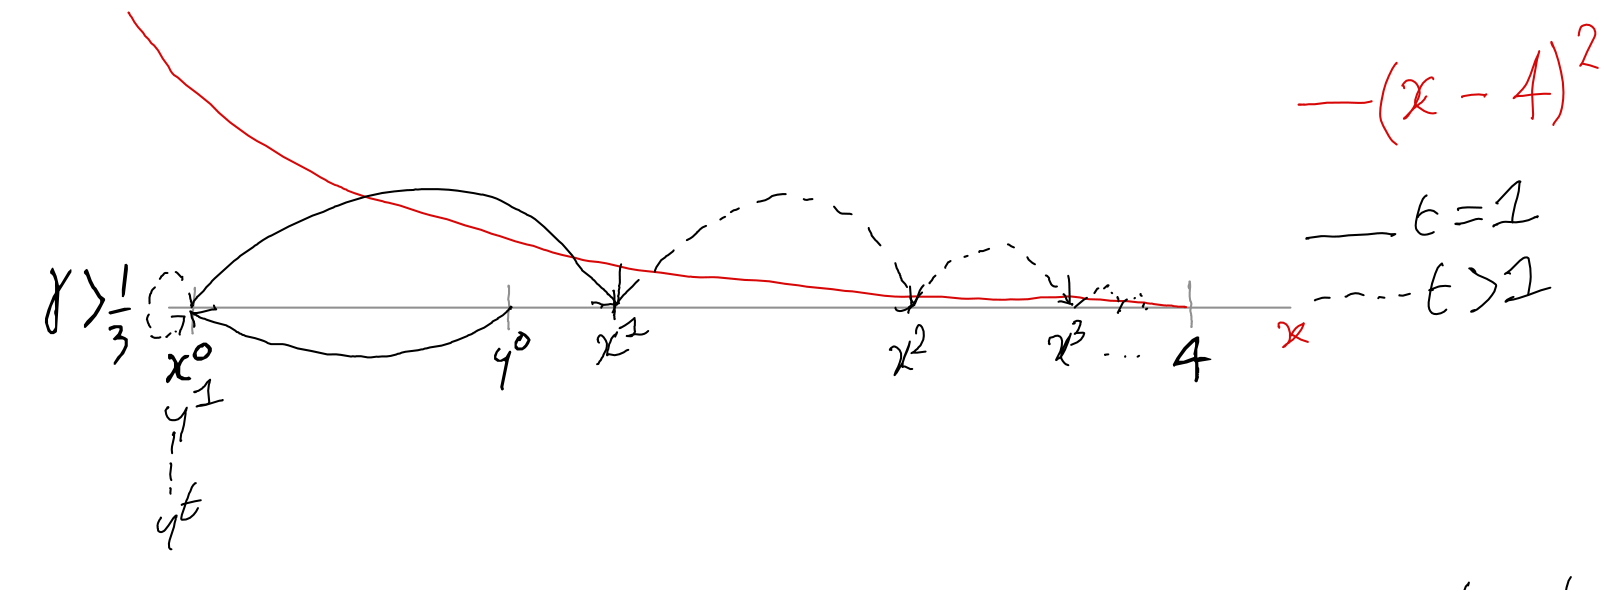
\includegraphics[width=0.7\textwidth]{imgs/schema_big_gamma.png}

On reprend \cref{eq:argwass} avec $t=1$ pour obtenir $(x,y)^{(t+1=2)}$. Les "positions initiales" sont maintenant $(x,y)^{(1)}$ calculé à la première étape:

\begin{equation}
	(x^{(1)}, y^{(1)}) = (1 + \frac{3}{1+\frac{1}{\gamma}}, \ 0)
\end{equation}

L'objectif étant convexe, l'optimal est toujours à droite de $x^{(1)}$, donc on a toujours $x > y^{(1)} = 0$.

\textbf{Cas 1. $\gamma < \frac{1}{3}$}

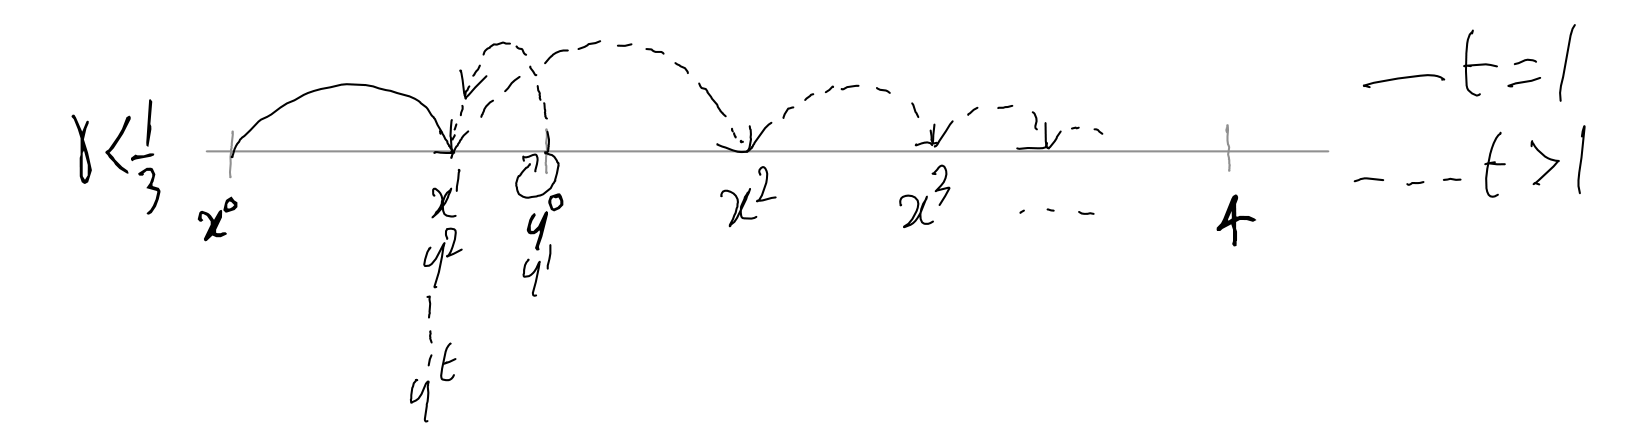
\includegraphics[width=0.7\textwidth]{imgs/schema_small_gamma.png}

$y$ est identique, $x$ se déplace vers 4. A un moment $t$, on aura $x^{t+1} > y^{0}$ ($\forall t' < t, \ y^t = y^0$) et on peut refaire les calculs de la première étape dans le cas $\gamma > 1/3$(on a juste $x$ différent).

\subsection{Extensions}

We can project the whole example into the first dimension of $\R^2$ and rotate it and we would find the same behavior.

Taking a ReLU network loss and weights, it seems unlikely that a problem with two neurons will have a \emph{different output} at convergence with the wasserstein distance.

However with many neurons we can still observe on the graph below, that in a single step of prox there are many exchanges being made, but in the end the two proxs will converge to the same solution.

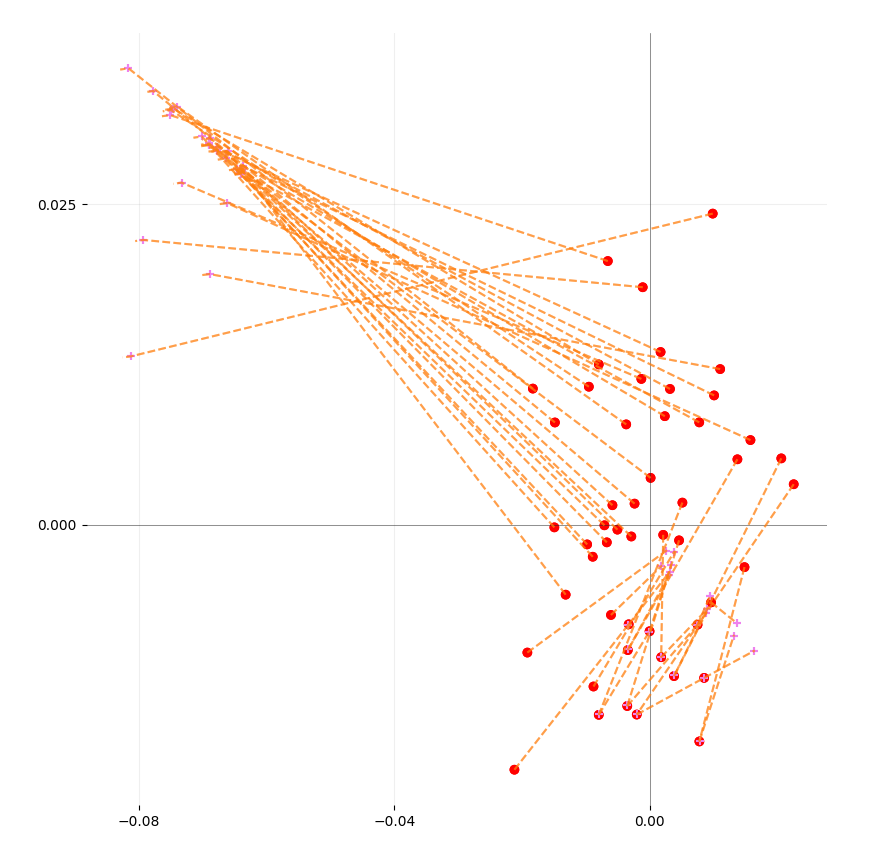
\includegraphics[width=0.7\textwidth]{imgs/graph_onlypositives.png}

This simulation is simply some random data that has two obvious directions:

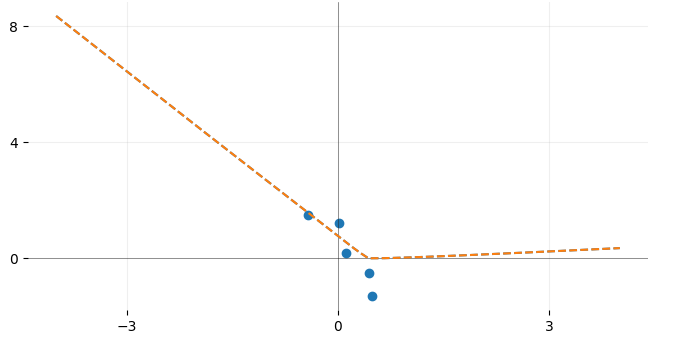
\includegraphics[width=0.7\textwidth]{imgs/graph_onlypositives_data.png}

To remove any suspicion we only considered positives neurons here. Indeed all previous simulations have allowed exchanges between positives neurons (that have +1 for the second layer and thus positive outputs) and negative neurons.

It is unclear if I should spend more time formalizing an example where we have an exchange.

\subsection{Next steps}

A 'large' stepsize for the proximal point using wasserstein might always happen in some scenarios with many neurons and a few obvious directions.

In practice it is not easy to see the difference in the converged network, in large neurons scenarios where the loss usually reach zero for both distances.

A large scale scenario will be ran (maybe many neurons in a grid again), with pos and neg distances computed differently (requires some code change).

\section{Prox point: Comparing the objective value and distance between iterates}
Which are the two items to minimize in proximal point.
\subsection{Early experiments}
\subsubsection{proximal point}

We run proximal point which optimize the objective $F(W^{t+1})$ and the distance between two iterates $d(W^{t+1)}, W^{(t)})$. We plot those two values for $\gamma=10$, and for Frobenius distance and Wasserstein distance as defined later.

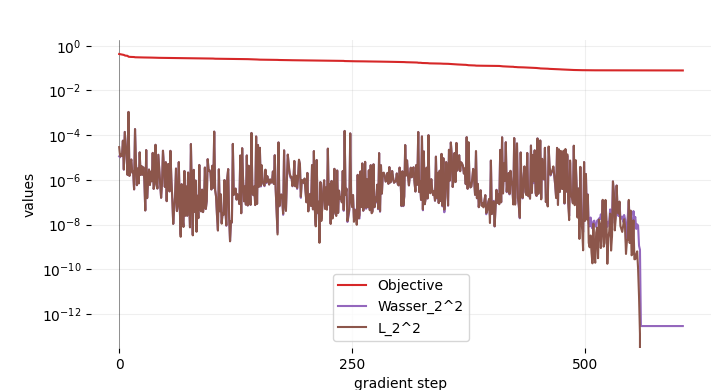
\includegraphics[width=0.7\textwidth]{imgs/tau10_graph_full.png}

It looks like they are exactly the same. We also plot the difference between the two distances to confirm.

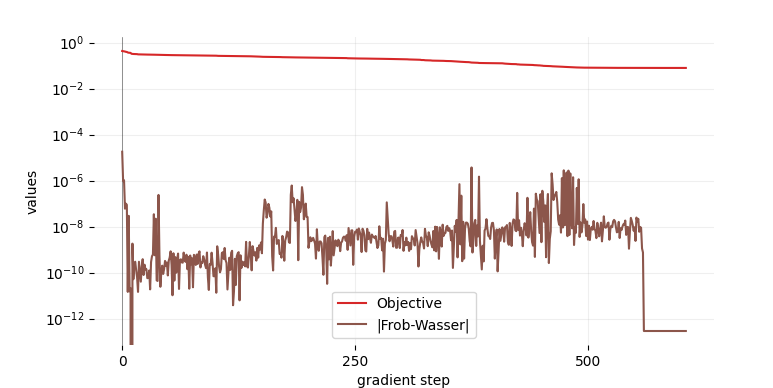
\includegraphics[width=0.7\textwidth]{imgs/tau10_graph.png}

Start and 'end' of convergence for proximal point:

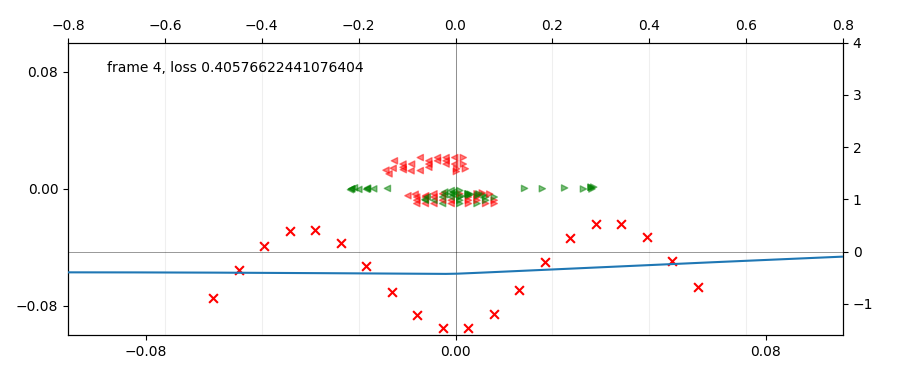
\includegraphics[width=0.7\textwidth]{imgs/tau10_plot_start.png}
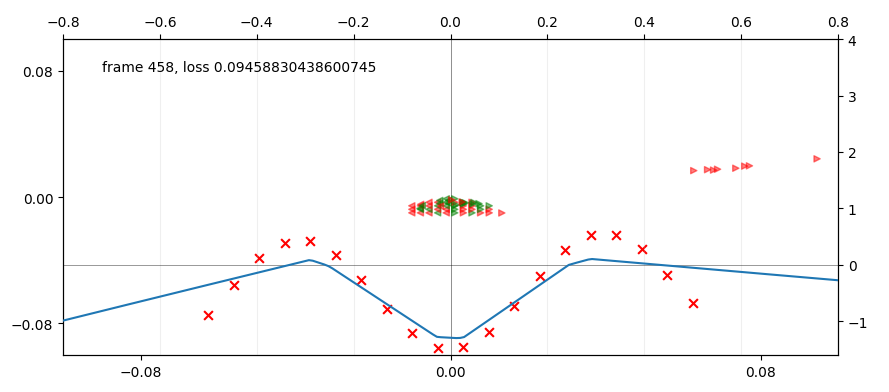
\includegraphics[width=0.7\textwidth]{imgs/tau10_plot_end.png}

It's a relatively large stepsize but not an easy problem. The triangle of neurons that do not move are simply neurons that do not activate any data. Initialization is a random grid, with an output norm close to zero.

\subsubsection{wasserstein descent}

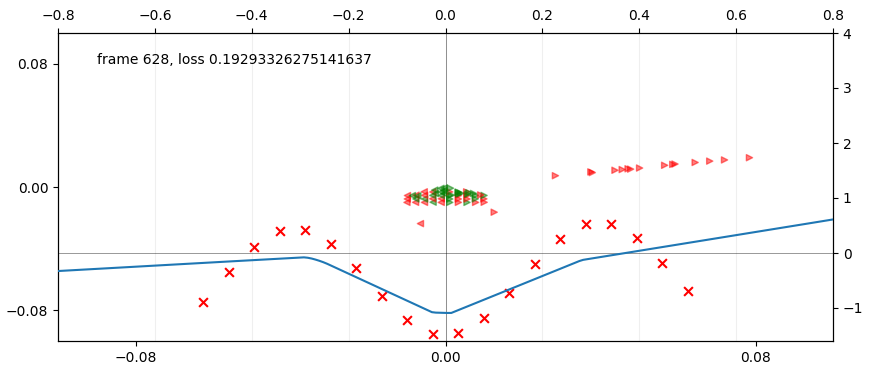
\includegraphics[width=0.7\textwidth]{imgs/tau10_plot_wasser_end.png}

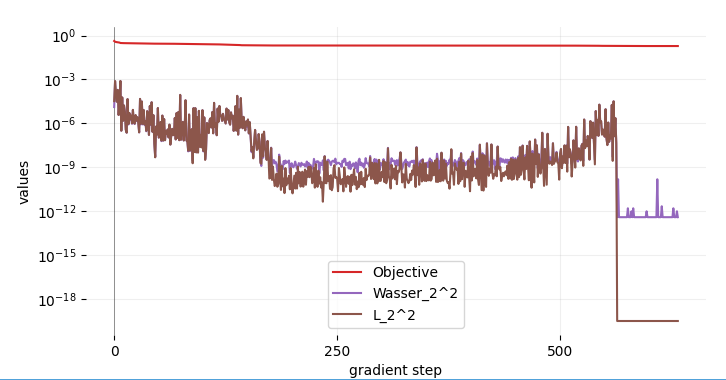
\includegraphics[width=0.7\textwidth]{imgs/tau10_graph_wasser.png}

The early trajectory is very similar, but then it looks stuck for a while.

Caveat: prox solution is not accurate due to small number of inner iterations.

\section{Larger simulations on Prox point}

$m = 50$(scale $10^{-2}$), $n = 5$(some usual $[-1, 1]$ sinus data), we compute $10^6$ prox inner iterations (the bigger the stepsize the larger the step size might need to be) for both the frobenius and the wasserstein distance. 

In blue/green filled lines we plot the normal MSE loss of the network (for frobenius proxpoint and wasserstein proxpoint)

In dotted/dashed lines we compute $d(W^{t)}, W^{(t+1)})$ (distance between iterates, which is one of the two objectives minimized at each step) for $d=$wasserstein and $d=$frobenius.

Because the only difference between wasserstein and frobenius is the assignement (which neuron/particle is assigned which particle to compute the distance), we also plot in thick green and red lines the number of permutations of the optimal mapping between two iterates. (1 = every particles has been permuted, 0 = each particle is associated to itself)

For $\gamma = 10^{-3}$ (small stepsize):

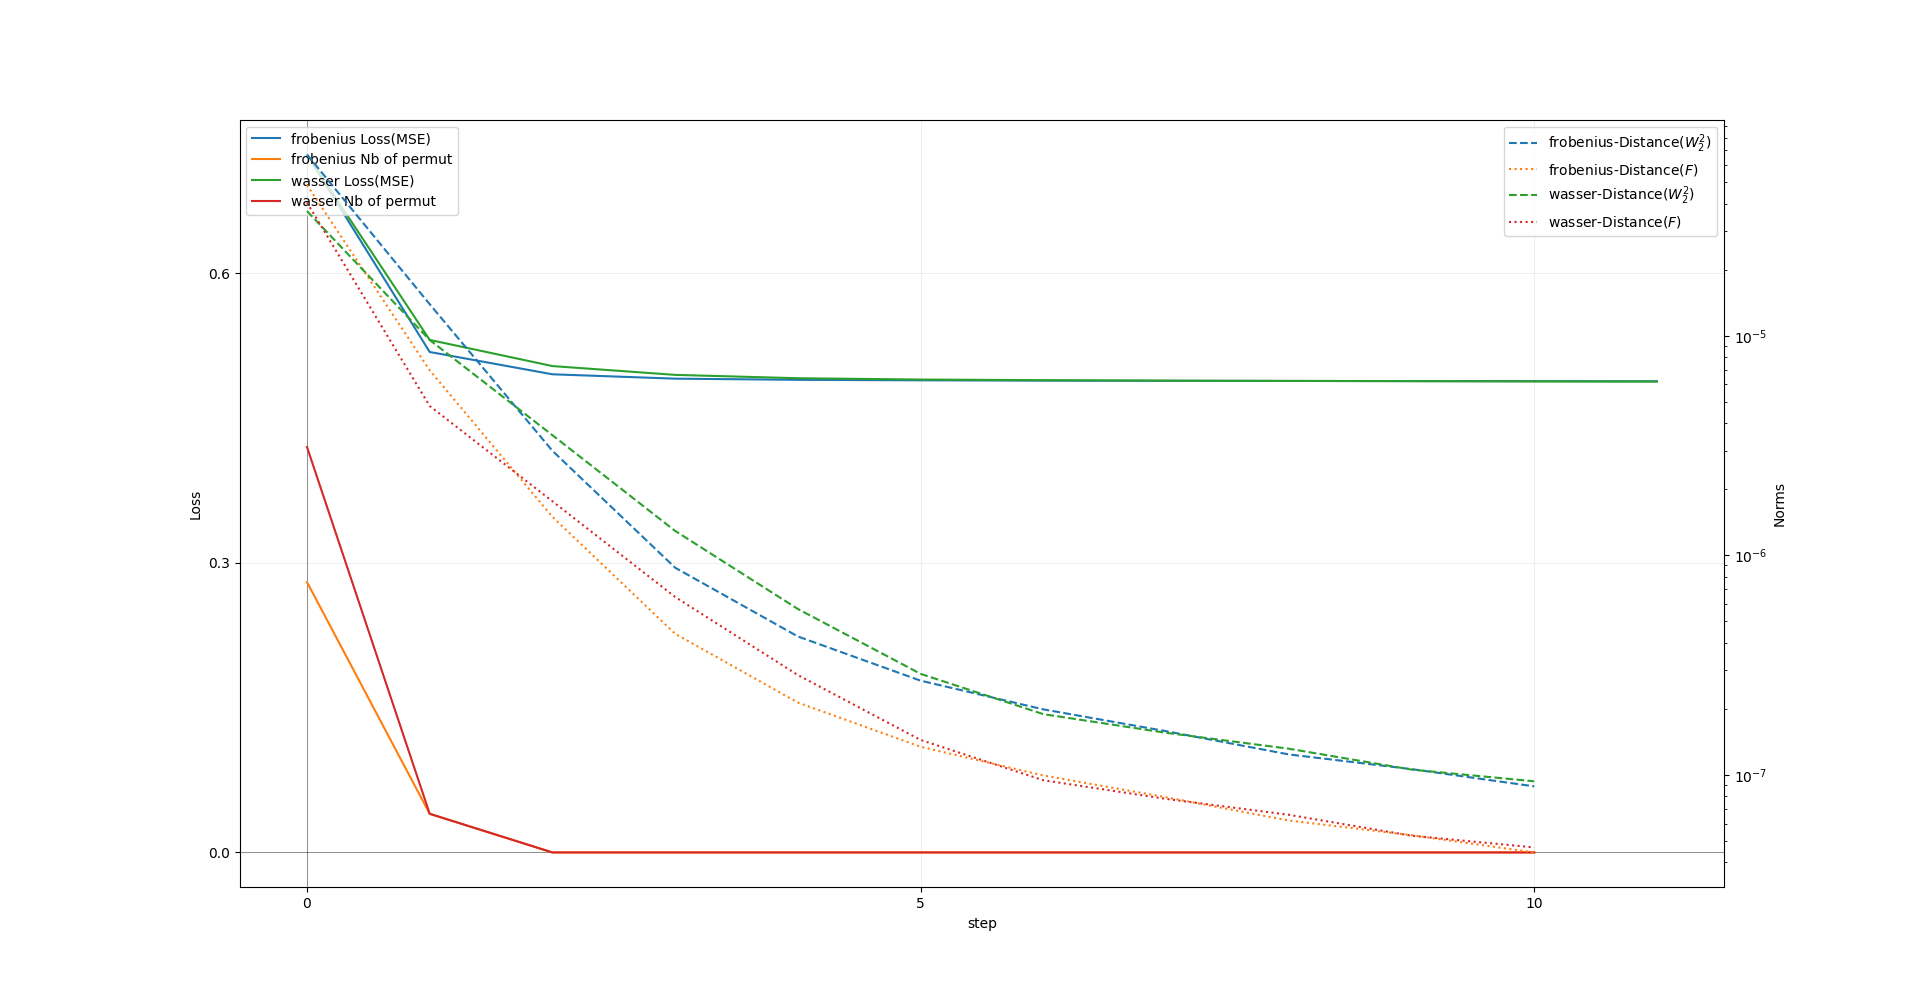
\includegraphics[width=1.0\textwidth]{imgs/petit_pas_10steps.png}

The 3 lines associated with wasserstein descent are very close to the 3 lines of frobenius descent, as expected.

For $\gamma = 10^0$ (big stepsize). This is one example where the convergence is very different. Wasserstein descent converges to 0 while Frobenius descent gets stuck on a bad local minima. We do the same plot as before.

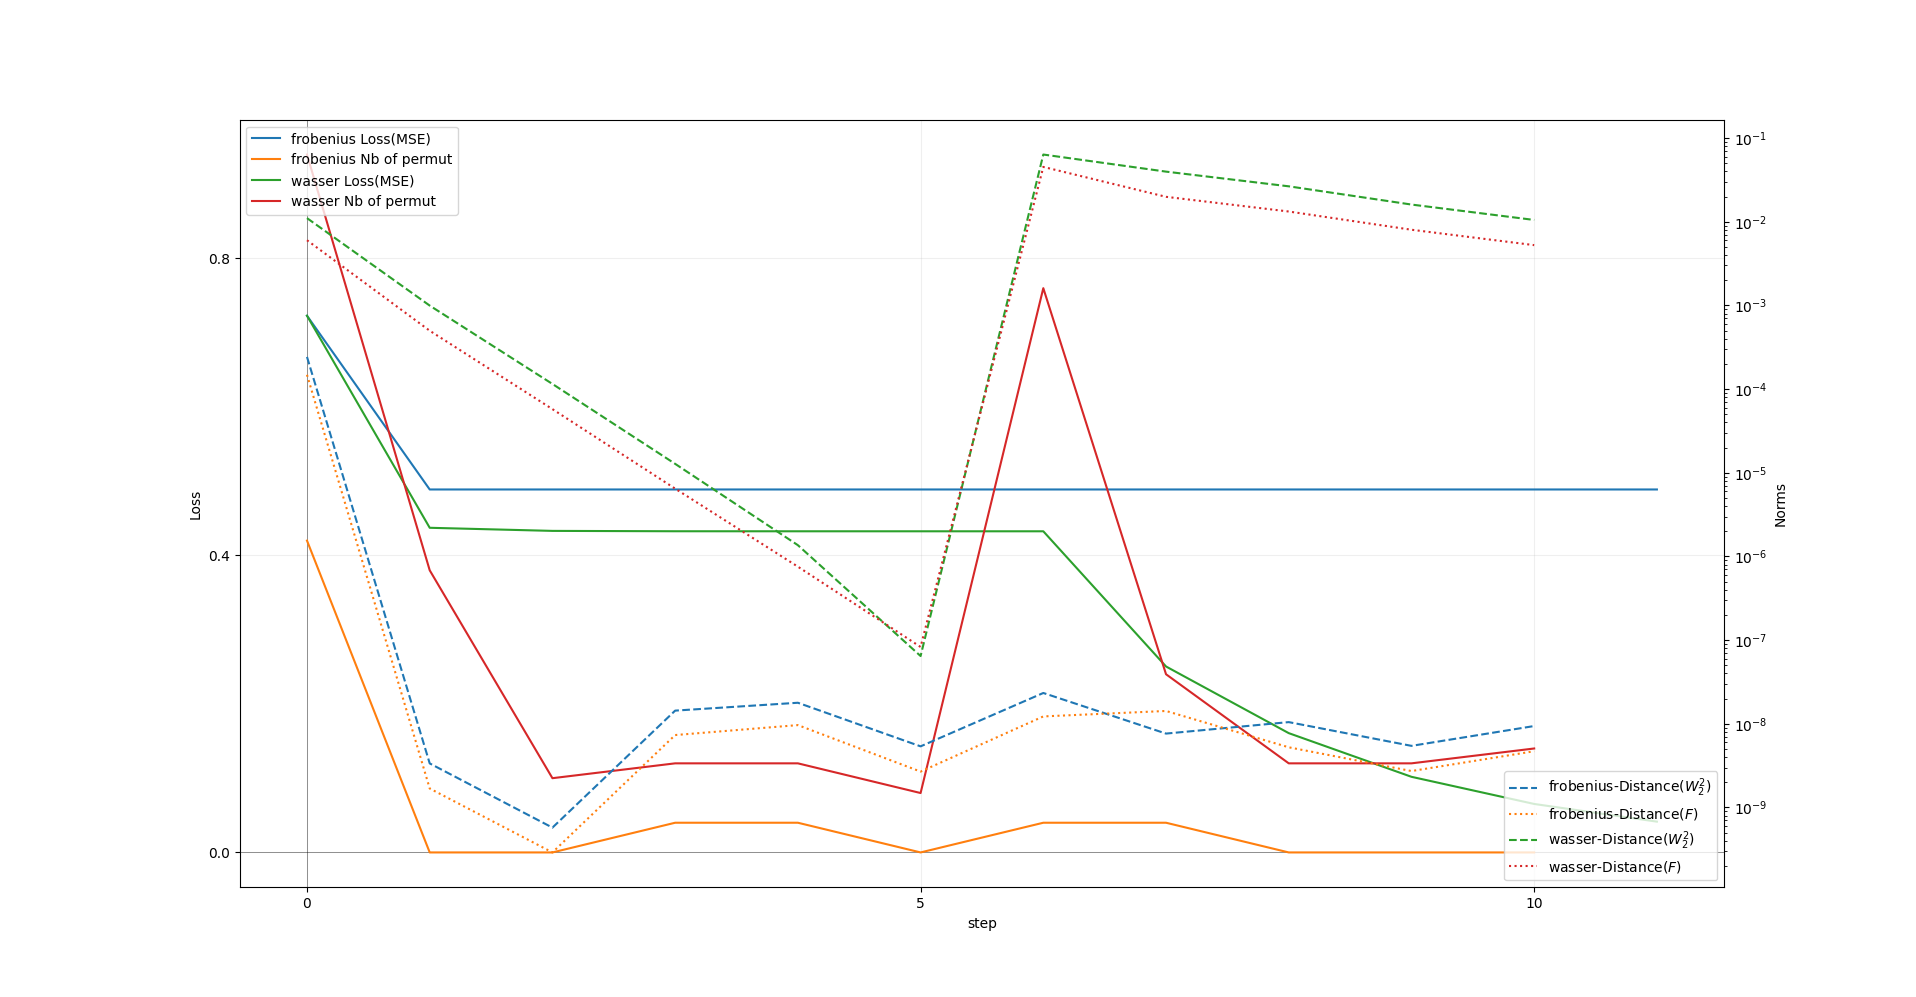
\includegraphics[width=1.0\textwidth]{imgs/grand_pas_10steps.png}

We can see the loss is completely different after 10 steps (it's normal to converge very quickly as the stepsize of the prox is large).

One thing to note, if we focus on wasserstein descent lines (dashed green and dotted red), the distance between iterates in frobenius or wasserstein is very close. However we can see in filled red that the number of permutations is close to 100\% at some steps.

This indicates that the actual distance value is not as important as the actual trajectories of the neurones which are decided by the gradient of the wasserstein distance used in the prox.

We plot the trajectories of each neuron (dashed lines for wasserstein descent and filled lines for frobenius descent) for the 10 prox steps. Circles denotes the initial positions of the neurons, blue for negative neurons and red for positives neurons.

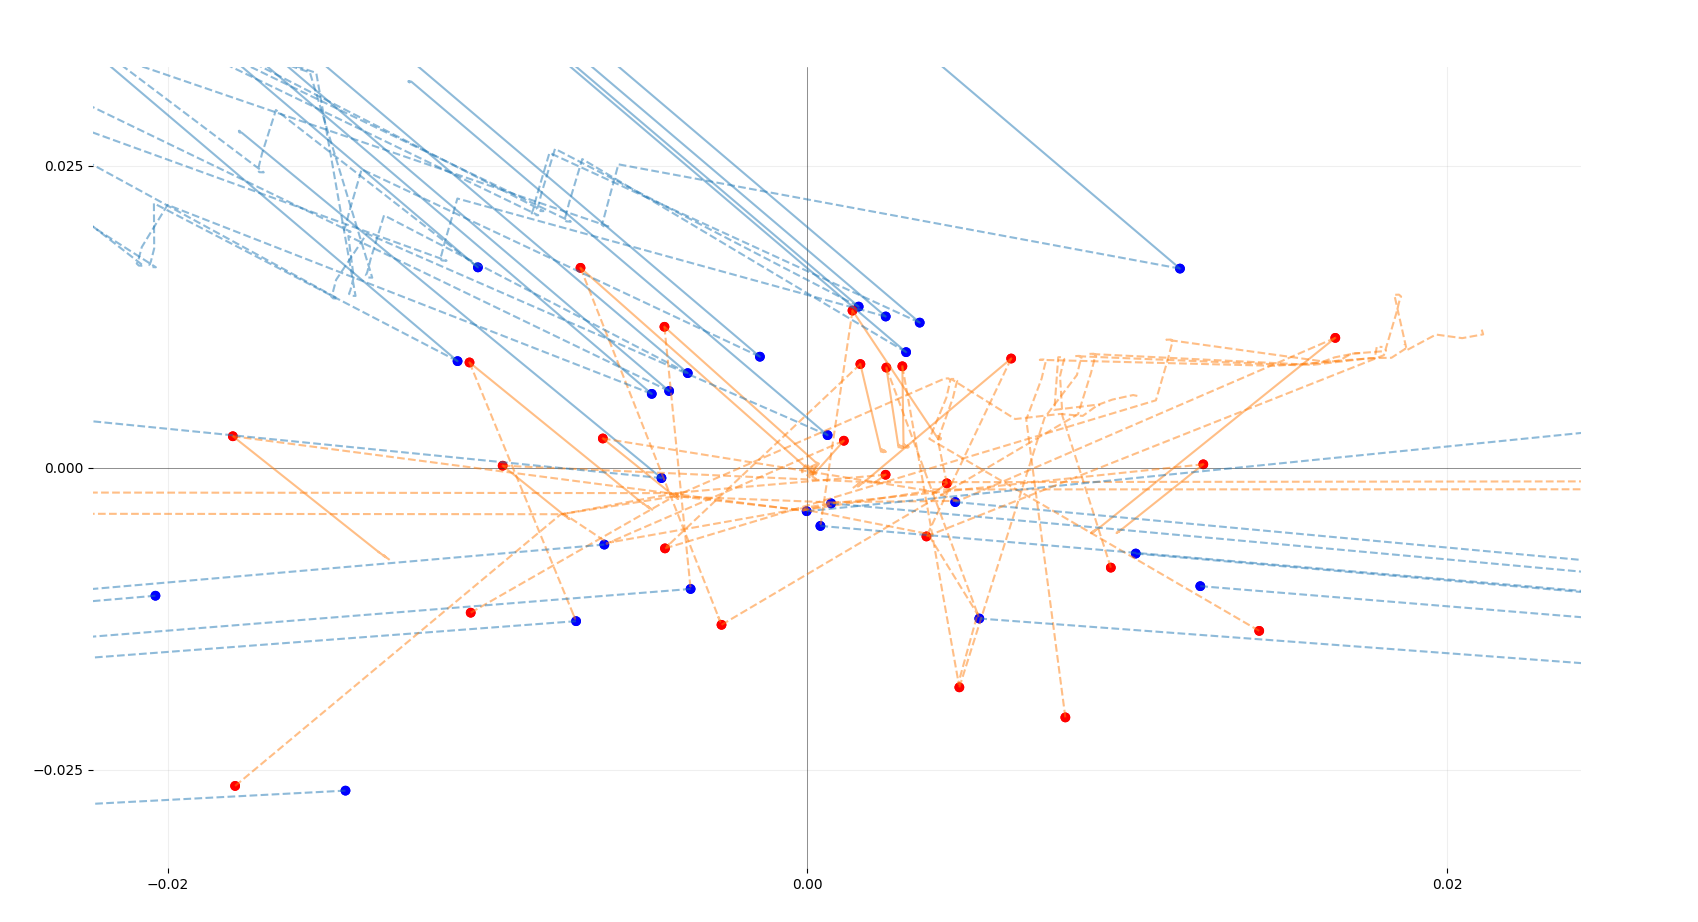
\includegraphics[width=1.0\textwidth]{imgs/grand_pas_10steps_trajs.png}

The trajectories are indeed different between the two descents. One major difference: neurons in the bottom quadrants are not moved at all by the frobenius descent, but in the wasserstein descent they are moved, they exchange positions (we can see two (dashed) trajectories very close going to and from the same initial neuron).

Those neurons (bottom/center quadrants) do not activate any datapoint and as such their differential is 0, so they cannot possibly move under prox descent. If weight decay is used, they will converge to 0. This completely differ from wasserstein descent, so the differential of the wasserstein distance must be different.

We'll focus on one proximal step by showing the first few \emph{inner} iterations for the two descents. We take two particles with different gradients. (this could happen near a non-differentiability, or as we see in the simulations if we can switch positive and negative neurons)

The inner iterations are dictated by the gradient of the objective $\frac{\partial F}{\partial w_i}$ to minimize the loss, and by gradient of the distance to the first iterate ($W^{(0)}$). The frobenius proximal point goes as usual, the distance gradient pulling the particle back to its initial position. However the wasserstein distance ends up pulling the particles to the other neuron's initial positions.

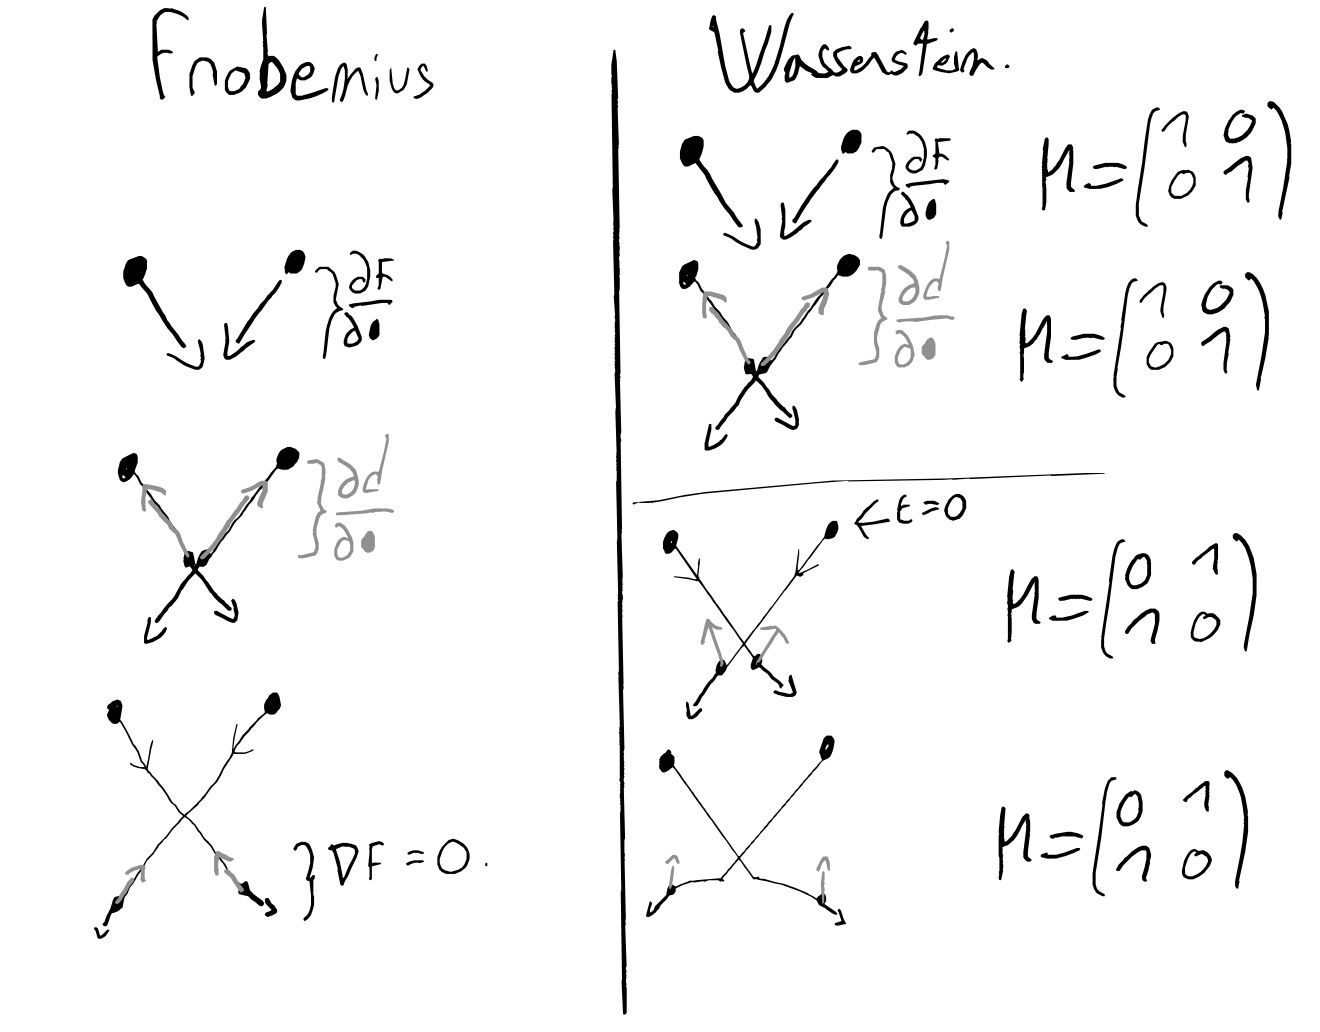
\includegraphics[width=0.7\textwidth]{imgs/schema_one_prox_step.png}

\emph{This explains a scenario where the prox will converge to something different. However it doesn't explain directly why the wasserstein prox can move neurons that have 0 gradient.}

Remark(not 100\% sure): in the mean field paper, the only results on ReLU are obtained by computing the wasserstein distance on two separate sets (i.e. you cannot assign a positive neuron to a negative neuron)


Implementations details: Frobenius is ran on one GPU(15min per run) while wasserstein is ran on a single CPU core (30min per run) as that was found to be the most efficient to run multiple experiments. Results for $\gamma=10^{a}$, $a=[0, -1, -2, -3, -4, -5]$ are available but do not differ much.

\section{Proximal point - direct WasserImplemented descents}

Discretized wasserstein prox step:

\begin{equation}
	W^{t+1} = \argmin_{W \in \R^{d \times m}} F(W) + \frac{1}{2 \step} W_p(W; W^t))
\end{equation}


EMD(POT library), d=squareeuclidian

\begin{align}
	W_2^2(W; W^t) &= \min_{\gamma} \inp{\gamma}{M}_F \\
	\text{s.t.  } \gamma ~ \mathbf{1} &= W \\
	\gamma^\top ~ \mathbf{1} &= W^t \\
	\gamma &\geq 0 \\
	M_{i, j} &= \lVert w_i - w_j \rVert^2_2
\end{align}

We only update the first layer $W^{(0)} \in \Theta = \R^{d \times m}$ for simplicity. $F : \Theta \rightarrow \R^+$ is the objective to minimize.

\begin{equation}
	\min_{W \in \Theta} \ F(W)
\end{equation}

\subsection{Gradient descent}

\begin{equation}
	W^{(t+1)} = W^{(t)} - \gamma \nabla F(W^{(t)}
\end{equation}

\subsection{Proximal point}

$d: \Theta \times \Theta \rightarrow \R^+$ a distance between two parameters

\begin{equation}
	W^{(t+1)} = \argmin_{V \in \Theta} \ \  F(V) + \frac{1}{2 ~ \gamma} ~ d(V, W^{(t)})
\end{equation}

To solve each $\argmin$, we use a gradient descent on $V$. $V^{(0)} = W^{(t)}$

\begin{equation}
	V^{(k+1)} = V^{(k)} - \beta \left(\nabla F(V^{(k)}) - \frac{1}{\gamma} \nabla d(V^{(k)}, W^{(t)})\right)
\end{equation}

\subsubsection{dist = L2 sq, frobenius}

Frobenius norm ($L_{2,2}$): $\norm{W}_{2,2}^2 = \norm{W}_F^2 = \sum_{i=1}^{m} \sum_{j=1}^{d} W_{i, j}^2 = \sum_{i=1}^{m} \norm{W_i}_2^2$

\begin{equation}
	d : (V, W) \in \Theta \times \Theta \rightarrow \frac{1}{m} \sum_{i=1}^{m} \norm{V_i - W_i}^2_2
\end{equation}

To sum up, we're solving this 

\begin{equation}
	W^{(t+1)} = \argmin_{V \in \Theta} \ \  F(V) + \frac{1}{2 ~ \gamma} ~ \frac{1}{m} \sum_{i=1}^{m} \norm{V_i - W_i}^2_2
\end{equation}

Using gradient descent for $\argmin$, one inner step (with inner step size $\beta$) on $V$ with $V^{(0)} = W^{(t)}$ is

\begin{equation}
	V^{(k+1)} = V^{(k)} - \beta \left(\nabla F(V^{(k)}) + \frac{1}{m ~ \gamma} (V^{k} - W^{(t)}) \right) 
\end{equation}

\begin{equation}
	V^{(k+1)} = V^{(k)}\left(1 - \frac{\beta}{m ~ \gamma}\right) + \frac{\beta}{m ~ \gamma} W^{(t)}   - \beta \nabla F(V^{(k)})
\end{equation}

which is kinda the same thing as this(only for $\gamma \rightarrow 0$) (trust region problem equivalence with proximal problem) $V^{(0)} = W^{(t)}$

\begin{equation}
	V^{(k+1)} = W^{(t)} - \gamma \nabla F(V^{(k)})
\end{equation}

\subsubsection{dist = wasserstein2 sq}

\textbf{distance definition.}
\begin{equation}
	W^{(t+1)} = \argmin_{V \in \Theta} \ \  F(V) + \frac{1}{2 ~ \gamma} ~ d(V, W^{(t)})
\end{equation}


With $V, W \in \R^d$ parameters.

p-Wasserstein distance between two measures $\mu, \nu \in \mathcal{P}(\R^d)$: 

\begin{equation}
	W_p(\mu, \nu)^p = \inf_{\gamma \in \Pi(\mu, \nu)} \int |y - x|^p \dd \gamma(x, y)
\end{equation}

$\Pi$ set of probability measures on $\R^d$ with marginals $\mu$ and $\nu$.

We take two sum of diracs measures $\mu = \frac{1}{m} \sum_{i=1}^{m} \delta_{V_i}$ and $\nu = \frac{1}{m} \sum_{i=1}^{m} \delta_{W_i}$. Then in that case $W_2$ is

\begin{equation}
	W_2(V, W)^2 = \min_{\sigma \in S_n} \frac{1}{m} \sum_{i=1}^{m} \norm{V_i - W_{\sigma(i)}}^2_2
\end{equation}

With $\sigma$ a permutation. This is the linear assignment problem which can be solved by the hungarian algorithm. It always has a solution so inf=min

This is equivalent to what \texttt{OT.emd(d=squareeuclidian)} solves:

\begin{align}
	W_2^2(W; W^t) &= \min_{\gamma} \inp{\gamma}{M}_F \\
	\text{s.t.  } \gamma ~ \mathbf{1} &= W \\
	\gamma^\top ~ \mathbf{1} &= W^t \\
	\gamma &\geq 0 \\
	M_{i, j} &= \lVert w_i - w_j \rVert^2_2
\end{align}

However, we only need the gradient of the distance. I haven't yet read what it is exactly.

\textbf{Small stepsize.}

To sum up, for wasserstein descent we have this step

\begin{equation}
	W^{(t+1)} = \argmin_{V \in \Theta} \ \  F(V) + \frac{1}{2 ~ \gamma ~ m} ~ \min_{\sigma \in S_n} \sum_{i=1}^{m} \norm{V_i - W_{\sigma(i)}}^2_2
\end{equation}

If $\gamma$ is small, the candidate $V$ will be close to $W^{(t)}$, and each $V_i$ will be close to $W^{(t)}_i$. Therefore the optimal assignment is the identity.

\begin{equation}
	W^{(t+1)} = \argmin_{V \in \Theta} \ \  F(V) + \frac{1}{2 ~ \gamma ~ m} ~ \sum_{i=1}^{m} \norm{V_i - W_i}^2_2
\end{equation}

Which is exactly the proximal point. Additionnaly, as the step size gets smaller, proximal point converges to the gradient flow (just like gradient descent).

\section{intuition on Small vs Big initialization in ReLU}

Why is it that as the scale gets smaller, the training dynamic consist of an alignment phase and then a convergence phase?

Notation: Take a neuron $w \in \R^d$. The norm of the neuron is $\norm{w}_2 = \sqrt{\sum_{i=1}^{d} w_i^2}$, the direction of a neuron is a vector of norm $1$: $\frac{w}{\norm{w}_2}$.

A training step is approximately $w^{(t+1)} = w^{(t)} + \gamma ~ \mathbf{v}$ with $\gamma$ a coefficient correlated with the current $(t)$ output, labels, error and step size. However, it is not directly correlated to the norm of the neuron.

$\mathbf{v} \in \R^d$ is a partial sum of training examples. It has its own norm and direction.

If $\norm{w^{(0)}}$ is large, $w^{(1)}$ will be close to $w^{(0)} + \gamma ~ \mathbf{v}$.

If $\norm{w^{(0)}}$ is close to 0, $w^{(1)}$ will be close to equal to $\gamma ~ \mathbf{v}$ as every coefficient of $w$ is negligible compared to the update. Therefore, its direction will (after some updates) be dominated by $\mathbf{v}$. The same for every neuron that activate the same data points. (Since activation pattern is entirely decided by direction, activation pattern will all converge to extremal vectors..)

Refs: (expés, some results) \citep{maennel2018gradient}, (the orthogonal paper) \citep{boursierGradientFlowDynamics2022}. (incremental learning) \citep{berthierIncrementalLearningDiagonal}, (scaling path) \citep{neumayerEffectInitializationScaling2023}.


\section{Math introduction}

\subsection{Gradient Flow}

Given a smooth function $a \rightarrow F(a)$, the gradient flow is gradient descent algorithm

$a^{l+1} = a^l - \gamma \nabla F(a^l)$

with a small enough $\gamma$. If $F$ is not smooth, the gradient flow is the proximal-point algorithm

$a^{l+1} = \prox^{||\cdot ||}_{\gamma F}(a^{(l)} = \argmin_a \frac{1}{2} \norm{ a - a^{(l)}}^2 + \gamma F(a)$

with a small enough $\gamma$.

If $F$ is defined on histograms, it makes sense to use the wasserstein distance $W^p$


%\section{3 points example}
%
%\begin{itemize}
%	\item Data: slope : $a = 2$
%	\item Data: $\begin{pmatrix} X_1\\X_2\\X_3\end{pmatrix} = \begin{pmatrix}x_1 & 1 \\ x_2 & 1\\x_3 & 1 \end{pmatrix}=\begin{pmatrix} 1 \\ 2 \\ 4 \end{pmatrix}  $, $Y = \begin{pmatrix}y_1\\y_2\\y_3 \end{pmatrix} = \begin{pmatrix}a x_1^1 \\ a x_2^1 \\ a x_3^1 \end{pmatrix} $
%	\item Loss: $F(W) = \frac{1}{2 n} \sum_{j=1}^{n} \left(\max(0, \inp{w_1}{X_j} \alpha_1  - y_j \right)^2$
%	\item Gradient: $\nabla F(W) = \begin{pmatrix} \frac{\partial F}{\partial w_1} \end{pmatrix} =
%		\frac{\alpha_1}{n} \sum_{j=1}^{n} e_j s_{1, j} X_j$
%	\item Algo: $W^{t+1} = W^t - \nabla F(W^t)$
%	\item Initialization: $W^0 = \begin{pmatrix} w_1\end{pmatrix} = \begin{pmatrix} 1 & 0\end{pmatrix} $, $\alpha = \begin{pmatrix} \alpha_1 \end{pmatrix}=\begin{pmatrix} 1 \end{pmatrix} $
%\end{itemize}
%
%Run gradient descent:
%
%\begin{itemize}
%	\item Iteration 0:
%	\begin{itemize}
%		\item $W^0 = \begin{pmatrix} 1 & 0\end{pmatrix} $
%		\item $s_1 = \begin{pmatrix} 0 \\ 0 \\ 0 \end{pmatrix} $
%		\item $e = \begin{pmatrix} \inp{w_1}{x_1} \alpha_1 - y_1 \\ \inp{w_1}{x_2} \alpha_1 - y_2\\ \inp{w_1}{x_3} \alpha_1 - y_3 \end{pmatrix} =
%			\begin{pmatrix}  \inp{\begin{pmatrix} 1 & 0 \end{pmatrix}}{\begin{pmatrix}1 & 1\end{pmatrix}} - 2 \\ \inp{\begin{pmatrix} 1 & 0 \end{pmatrix}}{\begin{pmatrix}2 & 1\end{pmatrix}} - 4\\ \inp{\begin{pmatrix} 1 & 0 \end{pmatrix}}{\begin{pmatrix}4 & 1\end{pmatrix}} - 8\end{pmatrix} =
%			\begin{pmatrix}1-2 \\ 2-4 \\ 4-8  \end{pmatrix} = \begin{pmatrix} -1 \\ -2 \\ -4 \end{pmatrix} $
%		\item $e_j = \inp{w_1}{X_j} \alpha_1 - y_j =  w_1^1 x_j + w_1^2 - a x_j = x_j (w_1^1 - a) + w_1^2$
%		\item $W^1 = \begin{pmatrix} w^1_1 & w^2_1 \end{pmatrix}  - \frac{1}{n} \sum_{j=1}^{3} (x_j(w^1_1 - a) + w_1^2) X_j$
%		\item $W^1 = \begin{pmatrix} w^1_1 & w^2_1 \end{pmatrix} - \frac{1}{n}\sum_{j=1}^{3} \begin{pmatrix} x_j^2 (w^1_1 - a) + x_j w^2_1 & x_j(w^1_1 - a) + w^2_1 \end{pmatrix}   $
%		\item $W^1 = \begin{pmatrix}w_1^1 -\frac{w_1^2}{n} (x_1 + x_2 + x_3) - \frac{(w_1^1 - a)}{n} (x_1^2 + x_2^2 + x_3^2)  & ok \end{pmatrix} $
%		\item $b = \frac{x_1 + x_2 + x_3}{n} = 7/3, c = \frac{x^2_1 + x^2_2 + x^2_3}{n} = 21/3 = 7$ % et beh la somme des carrés.
%		\item $W^1 = \begin{pmatrix}w_1^1 -w_1^2 b - (w_1^1 - a) c  &  w^2_1 - (w_1^1 - a) b + w^2_1\end{pmatrix} $
%		\item $W^1 = \begin{pmatrix}w_1^1 -w_1^2 b - w_1^1 c  + a c  &  w^2_1 - w_1^1 b + w^2_1 + a b \end{pmatrix} $
%		\item $W^1 = \begin{pmatrix} 1 - 0 -7 + 14 & 0 - 7/3 + 0 + 14/3 \end{pmatrix} = \begin{pmatrix} 8 &7/3 \end{pmatrix} $
%		\item $W^1 = W^0  + 7 \begin{pmatrix}  1 & \frac{1}{3}\end{pmatrix} $
%		\item $X_1 + 2 X_2 + 4 X_3 = \begin{pmatrix} 1+4+16& 1+2+4 \end{pmatrix} = \begin{pmatrix} 21 & 7 \end{pmatrix} = 7 \times 3 \begin{pmatrix} 1 & \frac{1}{3} \end{pmatrix}  $
%	\end{itemize}
%\end{itemize}

\section{JKO}

What we compute by using the entropic JKO flow iterations.

\begin{align}
	\forall t > 0, p_{t+1} := & \prox^{W_{\gamma}}_{\tau f}(p_t) \\
							= & \argmin_{p \in \text{simplex}} W_{\gamma}(p, q) + \tau f(p) \\
							= &\argmin_{p \in \text{simplex}}  \left( \min_{\pi \in \Pi(p, q)} \inp{c}{\pi} + \gamma E(\pi) \right) + \tau f(p)
\end{align}

\subsection{JKO stepping with Dykstra's algorithm}

-\verb|->| \href{https://arxiv.org/pdf/1502.06216.pdf}{Entropic WGF 2015}

\begin{align}
p_{t+1} := & \prox^{W_{\gamma}}_{\tau f}(p_t) \\
							= & \argmin_{p \in \text{simplex}} W_{\gamma}(p, q) + \tau f(p) \\
							= &\argmin_{p \in \text{simplex}}  \left( \min_{\pi \in \Pi(p, q)} \inp{c}{\pi} + \gamma E(\pi) \right) + \tau f(p)
\end{align}

Where $\pi$ is a mapping, $c$ the ground cost for every point on the grid. When the ground cost between two points in the euclidian space is $c_{i,j} = \norm{x_i- x_j}^2$, (and $\gamma=0$, $f$ smooth...), this scheme formaly discretize the above mentionned PDE.

To do the step above, we'll use a bregman splitting approach that replace the single implicit $W_\gamma$ proximal step by many iterative KL implicit proximal steps. Specifically(?) Dykstra's algorithm for JKO stepping. This involve using the gibbs kernel:$\xi = e^{-\frac{c}{\gamma}} \in \mathbb{R}^{N \times N}_{+, \ast}$


\begin{algorithm}
\caption{JKOstep}
\begin{algorithmic}[1]
\State $p \gets p_0 \in \R^m$
\State $q_{\text{norm}} \gets \lVert p \rVert^2$
\State $a, b \gets \mathbf{1}, \mathbf{1} \in \R^m$ \Comment{Initialize vectors with ones}
\For{$i \gets 1$ \textbf{to} $T$}
\State $p \gets \text{prox}^{\text{KL}}_{\tau/\gamma}(\xi b)$
    \State $a \gets p / (\xi b)$
    \State $\text{ConstrEven} \gets \frac{\lVert b \cdot (\xi a) - q \rVert}{q_{\text{norm}}}$
    \State $b \gets q / (\xi a)$
    \State $\text{ConstrOdd} \gets \frac{\lVert a \cdot (\xi b) - p \rVert}{q_{\text{norm}}}$
    
    \If{$\text{ConstrOdd} < \text{tol}$ \textbf{and} $\text{ConstrEven} < \text{tol}$}
        \State \textbf{break}
    \EndIf
\EndFor
\end{algorithmic}
\end{algorithm}
% $f$ "should" be convex and with a closed form proximal % from JKO paper.

\begin{itemize}
	\item \href{https://arxiv.org/pdf/2206.05262.pdf}{Meta Optimal Transport (paper)} and \href{https://github.com/facebookresearch/meta-ot}{(code git)}: InputConvexNN to predict solution of OT problem
	\item \href{https://arxiv.org/pdf/2106.06345.pdf}{JKOnet (paper)} and \href{https://github.com/bunnech/jkonet}{(code git)}:
		\begin{itemize}
			\item \href{https://github.com/bunnech/jkonet/tree/main/jkonet/models}{/models} \verb|->| sinkhorn loss defined in loss.py, differentiable loop in fixed point.py
			\item next step: trying to create the right \href{https://ott-jax.readthedocs.io/en/latest/_autosummary/ott.geometry.geometry.Geometry.html#ott.geometry.geometry.Geometry}{Geometry} object from OTT library, which is what's used for sinkhorn
		\end{itemize}
\end{itemize}



\subsection{Papers}


Paper with a \href{https://arxiv.org/pdf/1512.02783.pdf}{specific case that doesn't match ours:} 

\href{https://arxiv.org/pdf/2106.00736.pdf}{large-scale waserstein gradient flows} about computing WGF. They discretize over time, but not exactly space. They reformulate so that the argmin is over convex functions, and then discretize cvx functions using ICNN.

